%% ============================================================================
%% fig_2_5_hybrid_precedent.tex -- TikZ source of thesis Figure 6 (label
%% fig:hybrid_precedent, Ch.2). Each element follows the cited papers or the model code:
%%  (a) Hymba hybrid-head module: input projection -> attention heads || SSM heads
%%      (Mamba) -> norm, x beta_1 / norm, x beta_2 -> mean -> output projection
%%      (Hymba paper Eq. 3, Fig. 1a, p.17 "mean fusion").
%%  (b) Samba block: Mamba -> MLP -> SWA -> MLP, repeated in depth (Samba Fig. 1).
%%  (c) CLAM-TR: feature transform (Linear -> 512, ReLU, Dropout) -> gated attention
%%      over ALL N patches -> TopK keeps K = min(128, N) -> CLAM branch || retention
%%      branch (module by configuration) -> ADDITIVE fusion (+) -> Linear 512 -> 6.
%%      No concatenation, no LayerNorm at the fusion (thesis eq:fusion).
%% Sizes (KTU thesis guide, section 5.1: figure text >= 10 pt): every text item 10.1 pt
%% (the "+" 11 pt; math sub/superscripts at the standard 7 pt script size of 10 pt
%% text); the three panels are proportioned for that size, the two branch boxes of (c)
%% are as tall as the retention list needs, legend on two lines.
%% Natural width ~15.4 cm: include at \includegraphics[width=\textwidth] (scale ~1).
%% ============================================================================
\documentclass[border=1pt]{standalone}
\usepackage[T1]{fontenc}
\usepackage{newtxtext,newtxmath}
\usepackage{amsmath}
\usepackage{enumitem}
\usepackage{tikz}
\usetikzlibrary{positioning,arrows.meta,calc,decorations.pathreplacing}

% ---- sizes: printed >= 10 pt at scale ~1 (10.1 TeX pt = 10.06 bp) ----
\newcommand{\bodysize}{\fontsize{10.1}{12.4}\selectfont}
\newcommand{\plussize}{\fontsize{11}{13.4}\selectfont}
\DeclareMathSizes{10.1}{10.1}{7.07}{5.05}
\DeclareMathSizes{11}{11}{7.7}{5.5}

\definecolor{ink}{RGB}{28,36,58}
% fills separated by luminance so the code survives greyscale printing:
% attention ~0.79, fusion ~0.85, structured ~0.88, MLP/linear ~0.95, white 1.0
\definecolor{attnfill}{RGB}{186,208,238}
\definecolor{attnline}{RGB}{40,82,140}
\definecolor{ssmfill}{RGB}{252,220,180}
\definecolor{ssmline}{RGB}{170,92,20}
\definecolor{mlpfill}{RGB}{242,242,242}
\definecolor{mlpline}{RGB}{110,110,110}
\definecolor{fusfill}{RGB}{200,230,190}
\definecolor{fusline}{RGB}{48,116,48}
\definecolor{framec}{RGB}{185,185,185}
% legend swatch without a nested tikzpicture
\newcommand{\swatch}[2]{{\setlength{\fboxsep}{0pt}\setlength{\fboxrule}{0.5pt}%
  \fcolorbox{#2}{#1}{\rule{0pt}{7pt}\rule{14pt}{0pt}}}}

\begin{document}
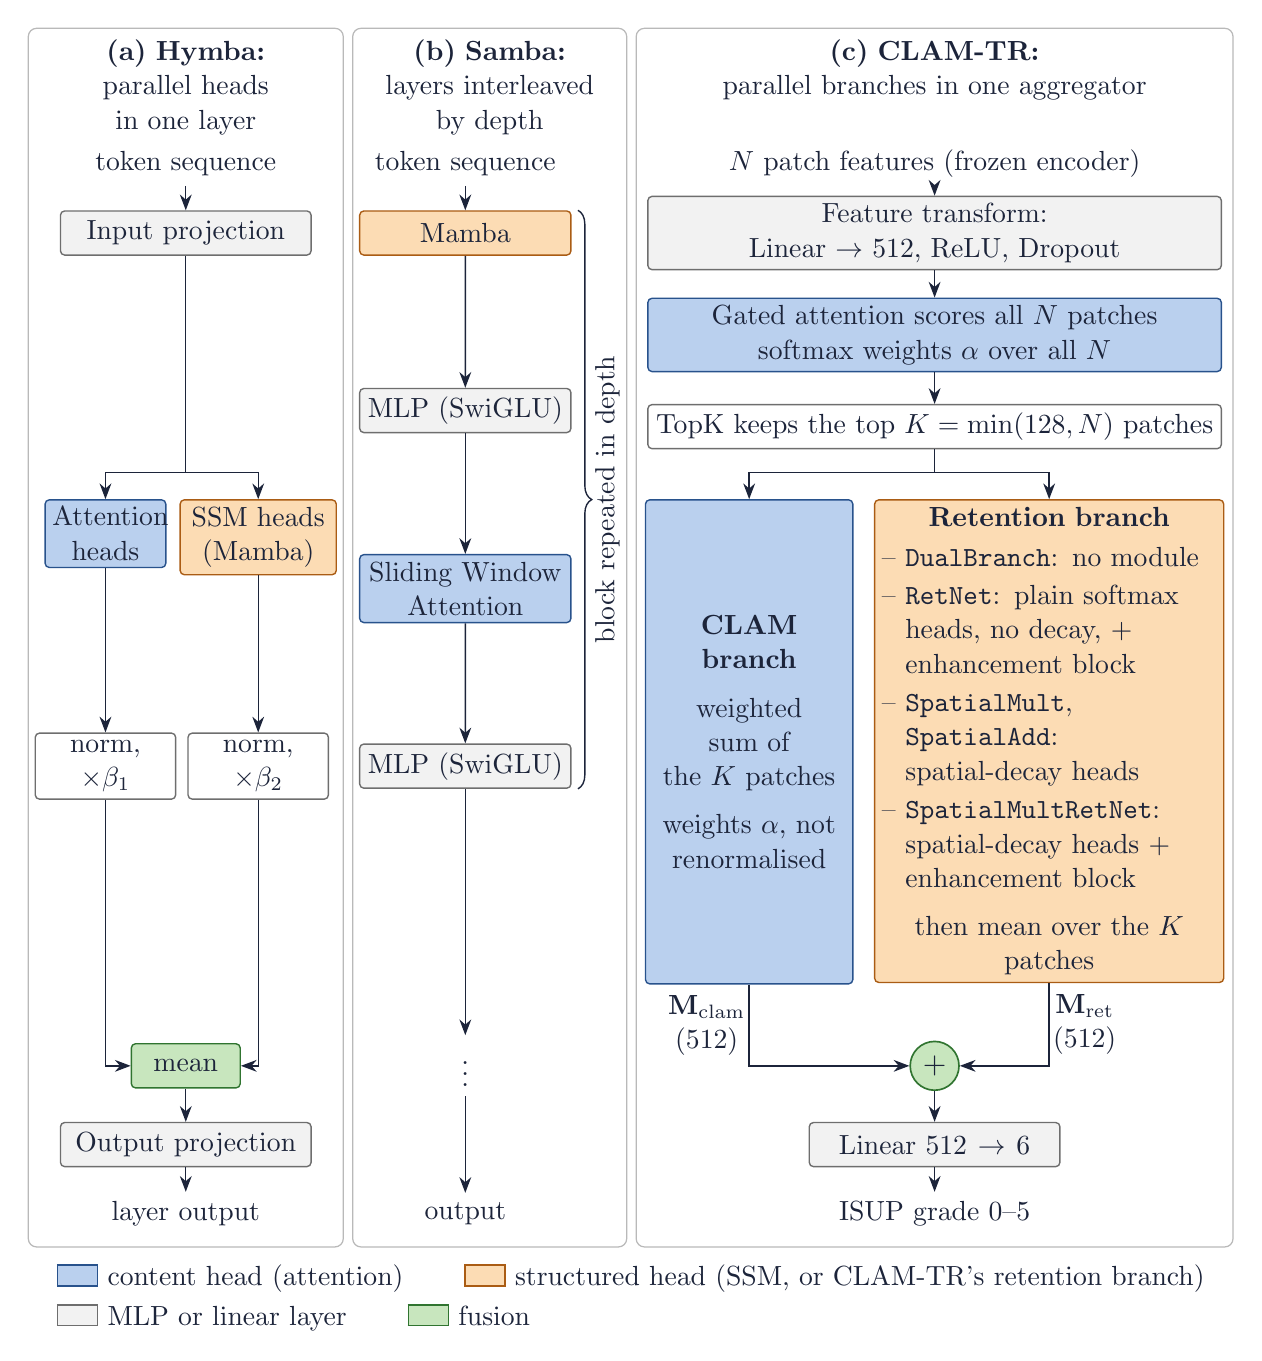
\begin{tikzpicture}[
  font=\bodysize, text=ink,
  every node/.append style={execute at begin node={\hyphenpenalty=10000}},
  >={Stealth[length=2.0mm,width=1.5mm]},
  box/.style={draw, rounded corners=1.5pt, align=center, line width=0.5pt,
              inner sep=2.6pt, minimum height=5.6mm},
  attn/.style={box, fill=attnfill, draw=attnline},
  ssm/.style={box, fill=ssmfill, draw=ssmline},
  mlp/.style={box, fill=mlpfill, draw=mlpline},
  plain/.style={box, fill=white, draw=mlpline},
  fus/.style={box, fill=fusfill, draw=fusline},
  ar/.style={->, line width=0.5pt, draw=ink},
  ln/.style={line width=0.5pt, draw=ink},
  lab/.style={inner sep=1.2pt},
  hd/.style={anchor=north, align=center, inner sep=0pt},
  panel/.style={draw=framec, line width=0.45pt, rounded corners=3pt}
]

% panels: (a) 0.00-4.00 | (b) 4.12-7.60 | (c) 7.72-15.30
\def\xa{2.00}
\def\xb{5.55}
\def\xc{11.51}
\node[hd, text width=3.80cm] at (\xa,-0.14) {\textbf{(a) Hymba:}\\ parallel heads in one layer};
\node[hd, text width=3.30cm] at (5.86,-0.14) {\textbf{(b) Samba:}\\ layers interleaved by depth};
\node[hd, text width=7.30cm] at (\xc,-0.14) {\textbf{(c) CLAM-TR:}\\ parallel branches in one aggregator};

% row heights shared by the panels (upper part); the lower rows follow the branch boxes of (c)
\def\yin{-1.72}   % input labels
\def\yA{-2.60}    % first processing row
\def\yj{-5.64}    % junction above the parallel stage
\def\ybr{-5.98}   % top of the parallel stage

% ============================== (c) CLAM-TR =================================
\node (inc) at (\xc,\yin) {$N$ patch features (frozen encoder)};
\node[mlp, text width=71mm] (ft) at (\xc,\yA)
  {Feature transform:\\ Linear $\rightarrow$ 512, ReLU, Dropout};
\node[attn, text width=71mm, anchor=north] (ga) at (\xc,-3.42)
  {Gated attention scores all $N$ patches\\
   softmax weights $\alpha$ over all $N$};
\node[plain, text width=71mm, anchor=north] (tk) at (\xc,-4.77)
  {TopK keeps the top $K=\min(128,N)$ patches};

\node[ssm, text width=42.5mm, anchor=north, align=left] (ret) at (12.965,\ybr)
  {\centering\textbf{Retention branch}\par
   \begin{itemize}[leftmargin=*, labelindent=0pt, labelsep=0.35em, itemsep=1.5pt,
                   topsep=2pt, parsep=0pt, partopsep=0pt, label={--}]
   \item \texttt{DualBranch}: no module
   \item \texttt{RetNet}: plain softmax heads, no decay, + enhancement block
   \item \texttt{SpatialMult}, \texttt{SpatialAdd}: spatial-decay heads
   \item \texttt{SpatialMultRetNet}: spatial-decay heads + enhancement block
   \end{itemize}
   \vspace{3pt}\centering then mean over the $K$ patches\par};
\path let \p1 = ($(ret.north)-(ret.south)$) in
  node[attn, text width=24.5mm, anchor=north, minimum height=\y1] (clam) at (9.155,\ybr)
  {\textbf{CLAM branch}\\[5pt] weighted sum of\\ the $K$ patches\\[5pt]
   weights $\alpha$, not\\ renormalised};

\coordinate (fu) at ($(ret.south)+(0,-1.05)$);   % fusion row
\coordinate (cl) at ($(fu)+(0,-1.00)$);          % projection / classifier row
\coordinate (ou) at ($(cl)+(0,-0.88)$);          % output labels

\node[circle, draw=fusline, fill=fusfill, line width=0.6pt, minimum size=6.2mm,
      inner sep=0pt, font=\plussize] (sum) at (\xc,0 |- fu) {$+$};
\node[mlp, text width=30mm] (cls) at (\xc,0 |- cl) {Linear $512\rightarrow 6$};
\node (outc) at (\xc,0 |- ou) {ISUP grade 0--5};

\draw[ar] (inc) -- (ft);
\draw[ar] (ft) -- (ga);
\draw[ar] (ga) -- (tk);
\draw[ln] (tk.south) -- (\xc,\yj);
\draw[ar] (\xc,\yj) -| (clam.north);
\draw[ar] (\xc,\yj) -| (ret.north);
\draw[ar] (clam.south) |- (sum.west)
  node[lab, align=center, pos=0.25, left] {$\mathbf{M}_{\mathrm{clam}}$\\ (512)};
\draw[ar] (ret.south) |- (sum.east)
  node[lab, align=center, pos=0.25, right] {$\mathbf{M}_{\mathrm{ret}}$\\ (512)};
\draw[ar] (sum) -- (cls);
\draw[ar] (cls) -- (outc);

% ============================== (a) HYMBA ===================================
\node (ina) at (\xa,\yin) {token sequence};
\node[mlp, text width=30mm] (ip) at (\xa,\yA) {Input projection};
\node[attn, text width=13.5mm, anchor=north] (att) at (0.98,\ybr) {Attention\\ heads};
\node[ssm,  text width=18mm, anchor=north] (ssmh) at (2.92,\ybr) {SSM heads\\ (Mamba)};
\coordinate (nr) at ($(clam.south)!0.45!(clam.north)$);  % norm row, inside the branch stage
\node[plain, text width=16mm] (n1) at (0.98,0 |- nr) {norm, $\times\beta_{1}$};
\node[plain, text width=16mm] (n2) at (2.92,0 |- nr) {norm, $\times\beta_{2}$};
\node[fus, text width=12mm] (mean) at (\xa,0 |- fu) {mean};
\node[mlp, text width=30mm] (op) at (\xa,0 |- cl) {Output projection};
\node (outa) at (\xa,0 |- ou) {layer output};

\draw[ar] (ina) -- (ip);
\draw[ln] (ip.south) -- (\xa,\yj);
\draw[ar] (\xa,\yj) -| (att.north);
\draw[ar] (\xa,\yj) -| (ssmh.north);
\draw[ar] (att) -- (n1);
\draw[ar] (ssmh) -- (n2);
\draw[ar] (n1.south) |- (mean.west);
\draw[ar] (n2.south) |- (mean.east);
\draw[ar] (mean) -- (op);
\draw[ar] (op) -- (outa);

% ============================== (b) SAMBA ===================================
\node (inb) at (\xb,\yin) {token sequence};
\node[ssm,  text width=25mm] (s1) at (\xb,\yA) {Mamba};
\node[mlp,  text width=25mm] (s2) at ($(s1)!0.333!(\xb,0 |- nr)$) {MLP (SwiGLU)};
\node[attn, text width=25mm] (s3) at ($(s1)!0.667!(\xb,0 |- nr)$) {Sliding Window\\ Attention};
\node[mlp,  text width=25mm] (s4) at (\xb,0 |- nr) {MLP (SwiGLU)};
\node (dots) at (\xb,0 |- fu) {$\vdots$};
\node (outb) at (\xb,0 |- ou) {output};

\draw[ar] (inb) -- (s1);
\draw[ar] (s1) -- (s2);
\draw[ar] (s2) -- (s3);
\draw[ar] (s3) -- (s4);
\draw[ar] (s4) -- (dots);
\draw[ar] (dots) -- (outb);
\draw[ln, decorate, decoration={brace, amplitude=5pt}]
  ($(s1.north east)+(0.08,0)$) -- ($(s4.south east)+(0.08,0)$)
  node[midway, right=5pt, rotate=90, anchor=north, inner sep=1pt]
  {block repeated in depth};

% ---------------------------------------------------------------- frames
\coordinate (fb) at ($(ou)+(0,-0.42)$);           % bottom of the panel frames
\draw[panel] (0.00,0) rectangle (4.00,0 |- fb);
\draw[panel] (4.12,0) rectangle (7.60,0 |- fb);
\draw[panel] (7.72,0) rectangle (15.30,0 |- fb);

% ============================== LEGEND ======================================
\node[inner sep=1pt, anchor=north, align=left] at ($(7.65,0 |- fb)+(0,-0.18)$)
  {\swatch{attnfill}{attnline}~content head (attention)\hspace{2.2em}%
   \swatch{ssmfill}{ssmline}~structured head (SSM, or CLAM-TR's retention branch)\\[2pt]
   \swatch{mlpfill}{mlpline}~MLP or linear layer\hspace{2.2em}%
   \swatch{fusfill}{fusline}~fusion};

\end{tikzpicture}
\end{document}
